\documentclass[journal,12pt,twocolumn]{IEEEtran}
\usepackage[utf8]{inputenc}
\usepackage{amsmath}
\usepackage{amssymb}
\usepackage{listings}
\usepackage{physics}
\newcommand{\myvec}[1]{\ensuremath{\begin{pmatrix}#1\end{pmatrix}}}
\let\vec\mathbf
\usepackage{graphicx}
\graphicspath{ {./images/} }

\title{Assignment 2
\\Probability }
\author{Swati Mohanty (EE20RESCH11007) }
\date{September 2020}

\begin{document}

\maketitle


\section{Problem}
A die is thrown three times. Events A and B are defined as below:
\\A : 4 on the third throw.
\\B : 6 on the first and 5 on the second throw.
\\Find the probability of A given that B has
already occurred?
\section{Solution}
Total sample space =216
\\Sample space of A (4 on the third throw) = 36
\\Sample space of B (6 on the first and 5 on  second throw) = 6
\begin{align}
    P(A) = \frac{36}{216}
    \\
    P(B) = \frac{6}{216}
    \\
P(A\cap B) = P(A) \times P(B)  
\\= \frac{36}{216} \times \frac{6}{216} = \frac{1}{216}
\\
    P(A | B) = \frac{P(A\cap B)}{P(B)}
    \\
    =\frac{\frac{1}{216}}{\frac{6}{216}} = \frac{1}{6} = 0.167
\end{align}
\section{Simulation}
In an experiment of throwing a fair die, the outcome can be any number from 1 to 6. So total sample space = \{1,2,3,4,5,6\}. If a die is thrown for three times, then total sample space = 6 \times 6 \times 6 = 216.
\\
Sample space = \{(1,1,1), (1,1,2),.....,(6,6,6)\(\)\}
\\
Each event in the sample space can be simulated by generating 3 random numbers between 0 to 6 and storing them into an array. \\
The frequency of event A from the simulated sample space = no. of times the last element of the generated array is 4 = a.
\[\implies P(A)= \frac{a}{total sample space}\]

The frequency of event B from the simulated sample space = no. of times the first and second element of the generated array are 6 and 5 respectively = b .
\[\implies P(B)= \frac{b}{total sample space}\]

Since event A and B are independent events, \[P(A\cap B) = P(A) \times P(B)\] .
Substituting the values in equation(5) we obtain the required probability.
\section{Result Analysis}
Theoretical probability = 0.167
\\Simulated probability = 0.162
\\Percetage of error obtained = 3.02%
\\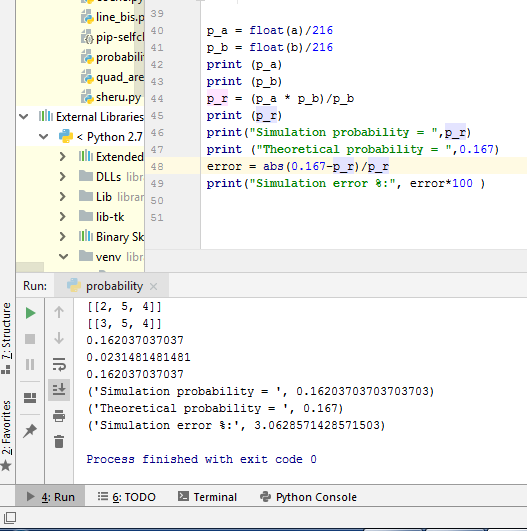
\includegraphics[width=9cm, height=9cm]{simulation result.png}
\\Python project link : 
https://github.com/Swati-Mohanty/EE5600/tree/master/Assignment%202

\end{document}